\documentclass[../../main.tex]{subfiles}

 \lhead{Project Management}
 
\begin{document}

\section{Project Management}
	\subsection{Management Methods}
	Upon starting the project, a simple Gantt chart was constructed to lay out the tasks that needed to be completed and the approximate time scale that should be allocated to each one. Very little of the project objectives changed from the initial planning other than one task which was producing low frequency accurate synthetic \ac{RIR}'s which would have taken a significant amount of time. This was removed from the project scope before the project implementation began and therefore was allocated no time.

	Two weeks into the project it was decided that the Gantt chart was not an appropriate method for project planning. This is because some tasks (such as producing synthetic \ac{RIR}'s) relied solely on the completion of the preliminary tasks. Once it was discovered that room modelling would take a lot longer than originally thought due to inexperience with such as task, the Gantt chart would have had to be redesigned which would have required even more time. Instead, a series of check lists were used to keep track of which tasks needed completing. These tasks were written on post-it notes and used in a large Kanban board situated on the authors bedroom wall, seen in figure~\ref{kanban}. This dynamic approach to project planning was much better suited to this project.  Along with this, weekly emails were sent to the projects supervisor with an update regarding the progress of the project and any problems that were faced, as well as regular meetings with both the projects supervisor and a larger group of students with audio related projects.

	Figure~\ref{gantt} in \nameref{appendixE} shows the initial Gantt chart with a red line indicating at what point it was abandoned for a more appropriate planning method.


	\begin{center}
	\begin{figure}
		\centerline{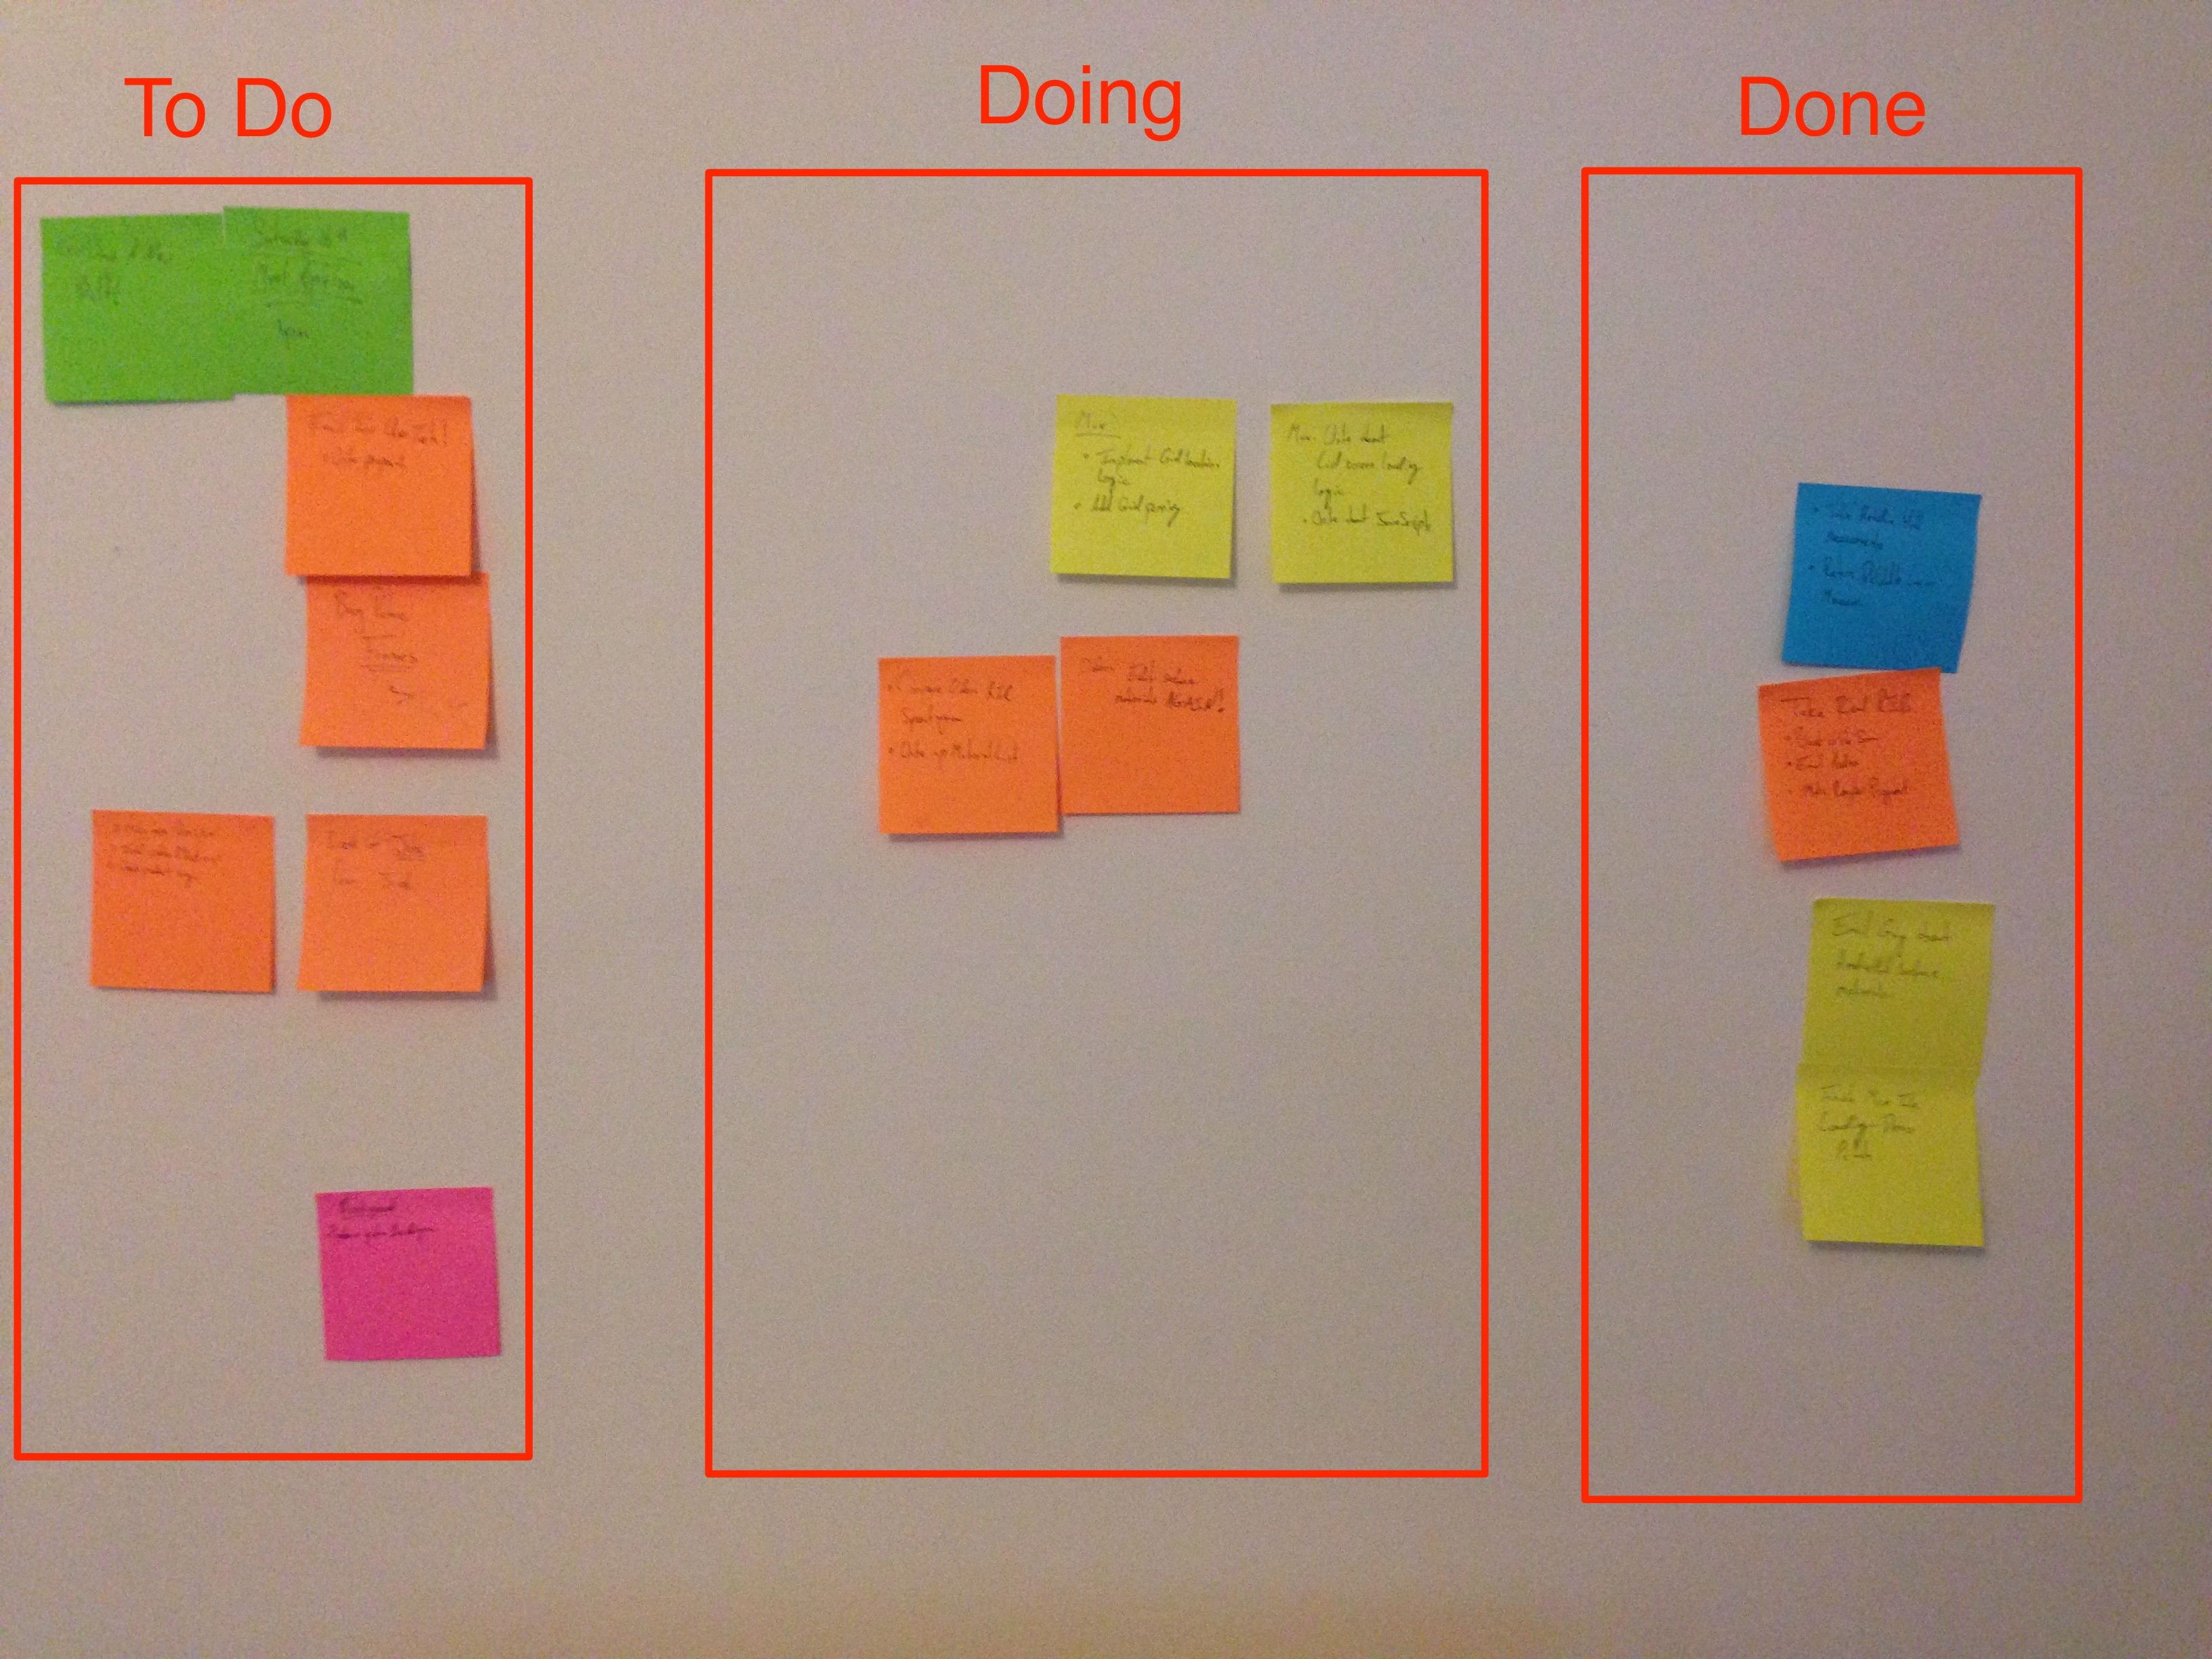
\includegraphics[scale = 0.15]{Sections/ProjectManagement/images/kanban_edit.jpg}}
		\caption{Image of the Kanban board used for keeping track of which tasks needed doing, which ones were ongoing and which tasks had been completed. This image was taken mid-way through the project.}
		\label{kanban}
	\end{figure}
	\end{center}

	\subsection{Dealing With Issues}

		When issues arose in the project that were unexpected therefore consuming unallocated project time, time limits on fixing issues were set. An example of this is the software implementation. When the issue arose where the originally designed system (\nameref{iteration1}) did not work as intended, a compromise had to be found. However, as the majority of the time had been put into designing the original software patch, there was little time left to design the second. Due to this, the final implementation of the software does not work exactly as intended, however setting the time limit allowed for a system to be built that could be used for the user tests, as opposed to improving the system further but not being able to complete the user tests. It was found that sacrificing the quality of certain aspects in the project (such as the software) allowed for the completion of the project and a more thorough analysis of the project process as a whole.

	%Decisions were made when to move on from an issue. This was the case when implementing the Max patch, when iteration 1 would not work and there was not alot of time left to implement the system, iteration 3 was build. This allowed me to fulfil the main aim, which is to produce a system that allows the user to move around the space, however it effected the quality of the user test results.


\end{document}